\chapter{Nuevos operadores para STL}
\label{cha:stl}

\section{Signal Temporal Logic}
% Definición, sintaxis y semántica de los operadores.
\textit{Signal Temporal Logic} (STL) \cite{STL} es un tipo de lógica temporal especializada en el análisis de señales reales analógicas. STL permite expresar características sobre la evolución de algún atributo físico, como la velocidad o temperatura. Por tanto, como punto de partida, STL requiere una muestra o traza de ejecución sobre la que comprobar las hipótesis.

La lógica distingue dos tipos de situaciones: propiedades que se satisfacen en un \textit{estado} o momento puntual de la traza de ejecución, o propiedades de \textit{camino} que se evalúan a lo largo de una secuencia de eventos. STL proporciona operadores para recorrer los diferentes estados del sistema y comprobar en qué momentos se cumplen las propiedades.

Por ejemplo, la proposición atómica $v > 120$ mostraría los instantes en los que la velocidad supera los $120$. Los operadores de camino enriquecerían esa expresión para analizar si la velocidad se sobrepasa puntualmente en algún momento (\textbf{F})uturo del viaje, (\textbf{G})eneralmente a lo largo de todo el recorrido, o permanece constante hasta (\textbf{U}ntil) que se incrementa a un nuevo valor. 

Formalmente, la gramática básica de STL comprende los siguientes operadores:

$$ \varphi \ := \ \mu \ |\ \neg \varphi \ |\ \varphi_{1} \lor \varphi_{2} \ |\ \varphi_{1} U_{[a,b]} \varphi_{2}$$

Donde $\mu$ representa las proposiciones atómicas, en forma de desigualdades sobre la señal muestreada; y $\varphi$ las especificaciones sobre los caminos. El resto de los operadores se componen a partir de los operadores precedentes, donde $a, b \in \mathbb{R}$ son marcas temporales que definen el intervalo de monitorización respecto al instante inicial (0). 

% Operador futuro y general

$$ F_{[a,b]} \varphi \equiv \top U_{[a,b]} \varphi $$
$$ G_{[a,b]} \varphi \equiv \neg F_{[a,b]} \neg \varphi $$
Existen versiones extendidas que permiten analizar aspectos cuantitativas con STL, por ejemplo, los valores máximos/mínimos \cite{TACAS_19} o integrales en un intervalo, o calcular la derivada en un punto \cite{Stl_Der_Int}.


Las especificaciones en STL se \textit{compilan} en un monitor que supervisa la ejecución del sistema (p. ej., el sensor de velocidad de un vehículo). Algunos intérpretes de STL son AMT \cite{AMT2} (sintaxis básica) y STLEval \cite{StlEval} (sintáxis básica + operadores de min/max). En este proyecto, implementaremos en STLEval los operadores cuantitativos de STL que permiten calcular integrales y derivadas sobre una señal, según la definición propuesta en \cite{Stl_Der_Int}.

\section{STLEval}
%Lenguaje utilizado en STLEval (C++), etc.

% Muestreo de la señal. Representación interna en STLEval.
La imagen \ref{fig:senal} ilustra la señal original y su representación interna en STLEval. 

\begin{figure}
\centering
  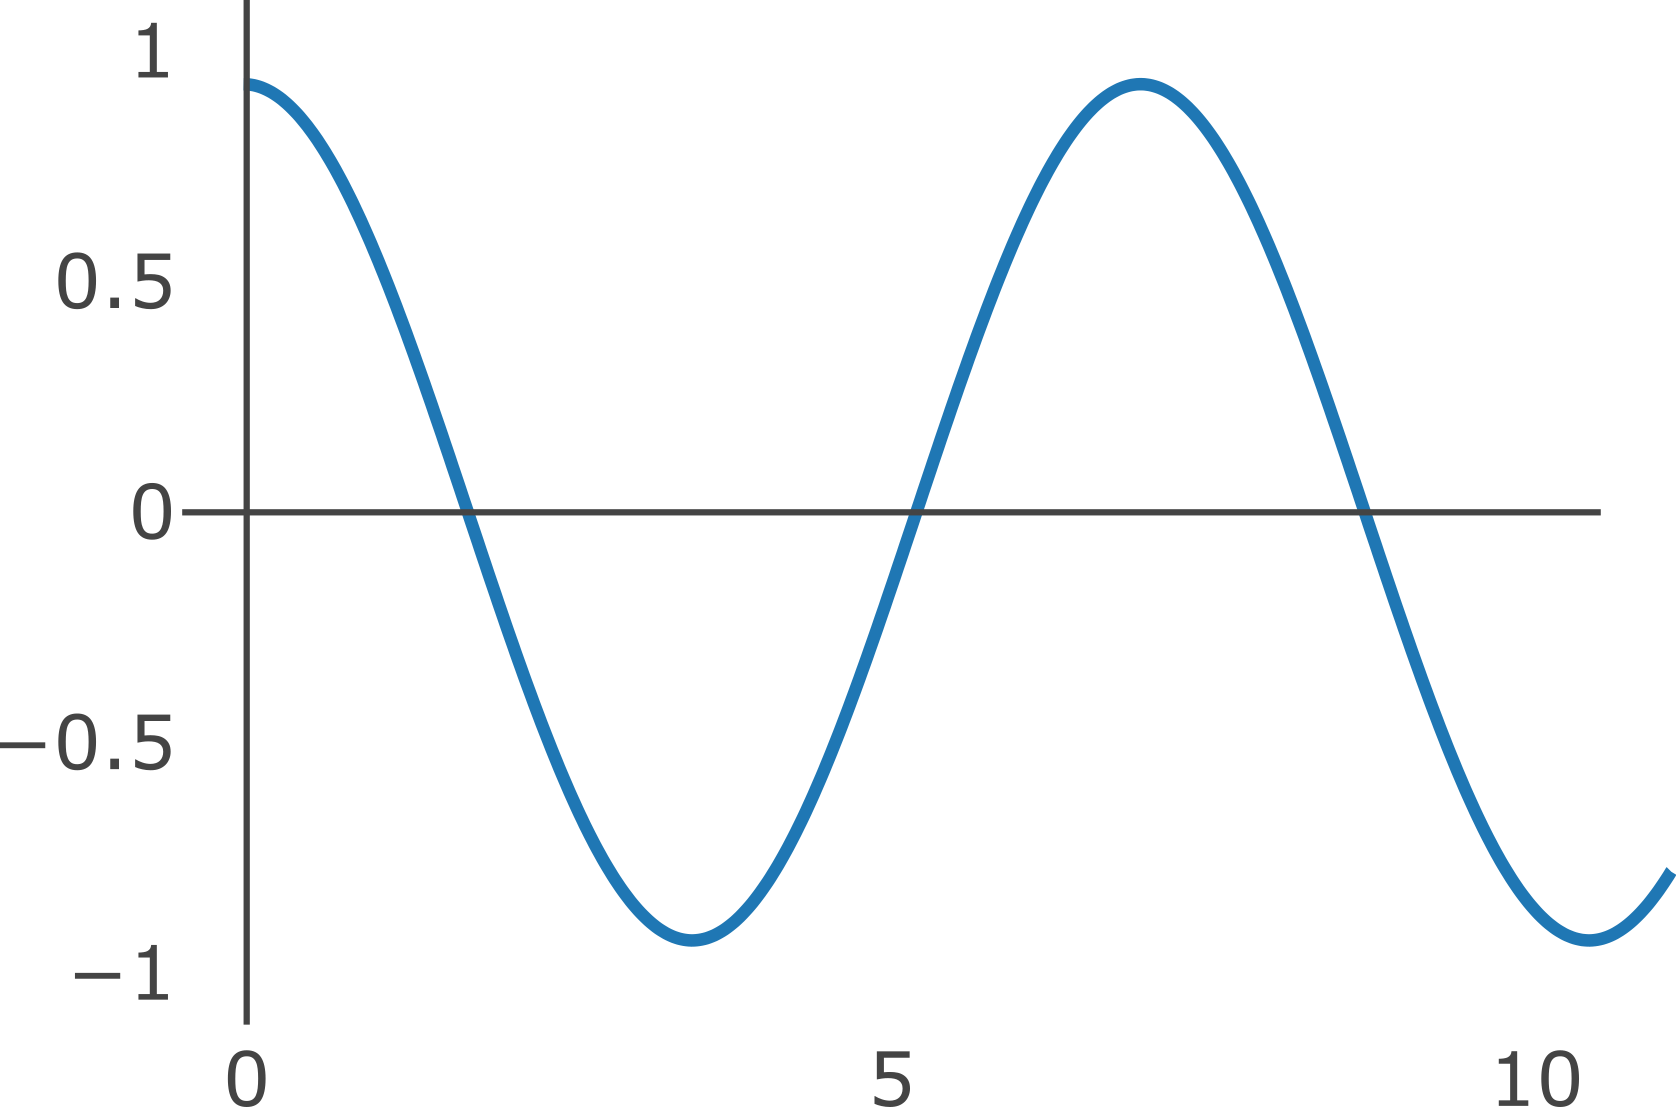
\includegraphics[width=.4\linewidth]{images/senal_original} \hfill
  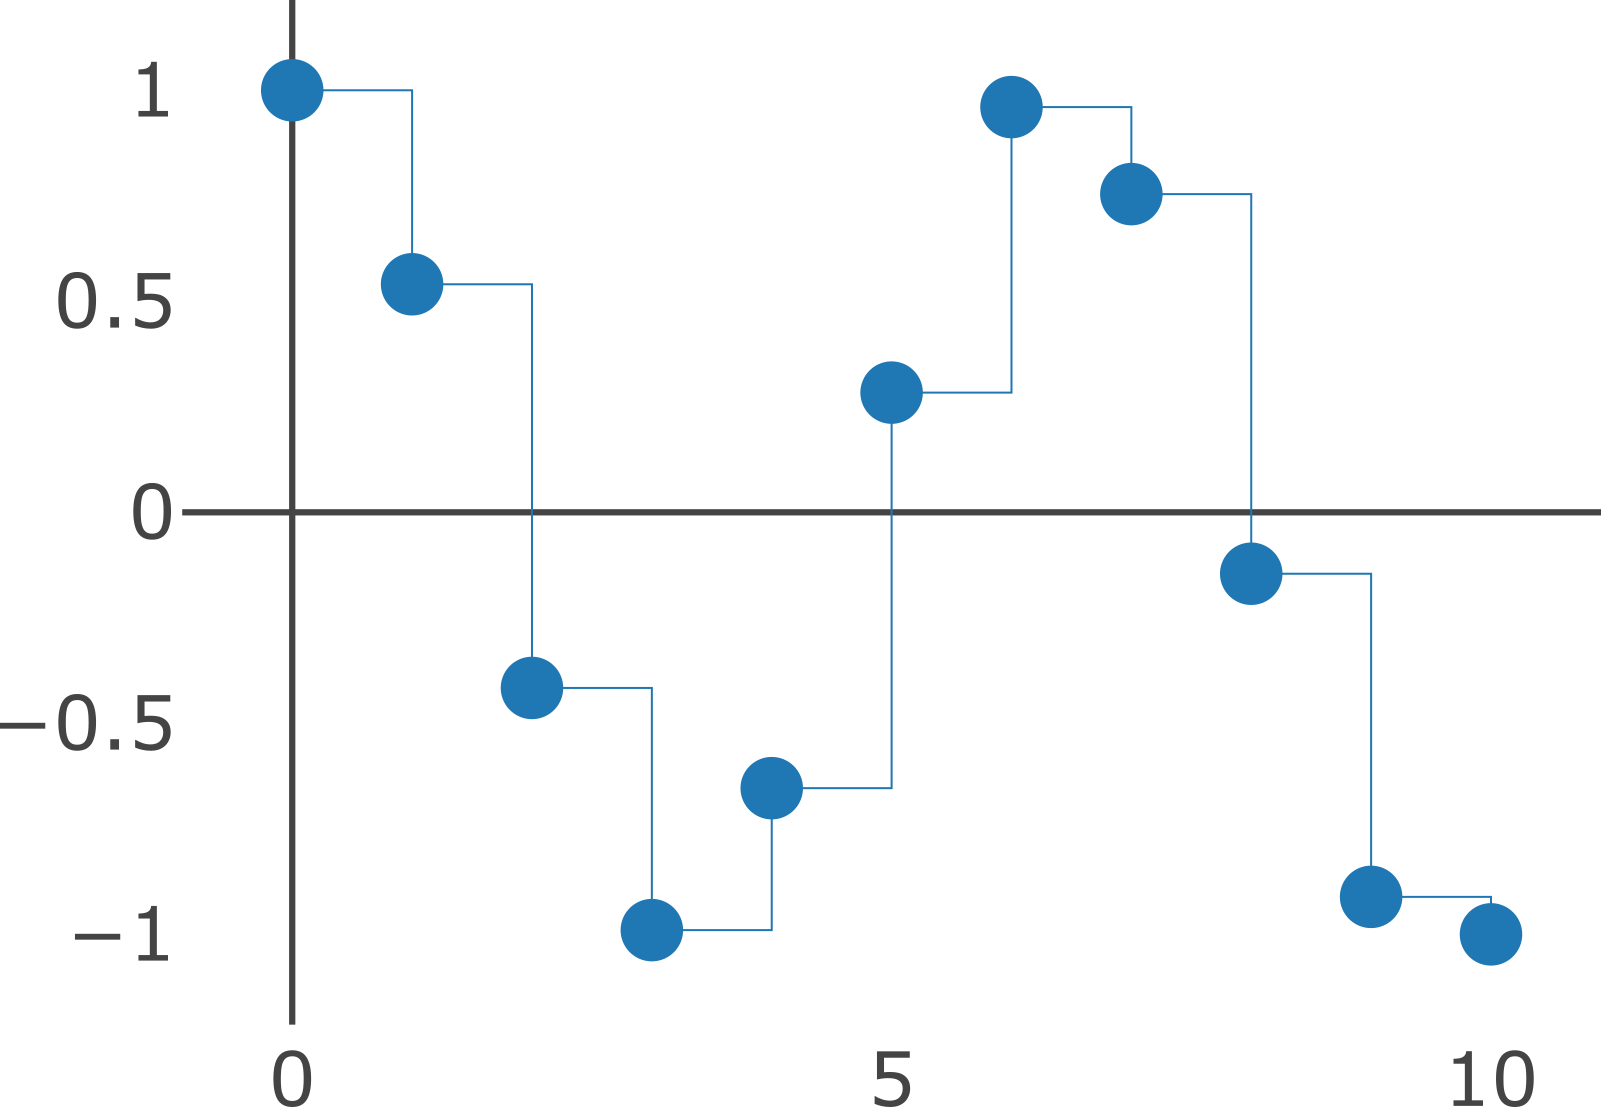
\includegraphics[width=.4\linewidth]{images/senal_muestreada}
\caption{Señal original y su reconstrucción.}
\label{fig:senal}
\end{figure}

\subsection{Operador integral}

El cálculo de la derivada e integral se aproximan mediante las siguientes expresiones matemáticas:

%TODO:
%Rescatar los sumatorios del PDF referenciado en la cita anterior.

Gráficamente, la derivada se interpreta como la pendiente entre dos puntos de la señal; y la integral como el sumatorio de los rectángulos contenidos (Figura \ref{fig:der_int}).

\begin{figure}
\centering
  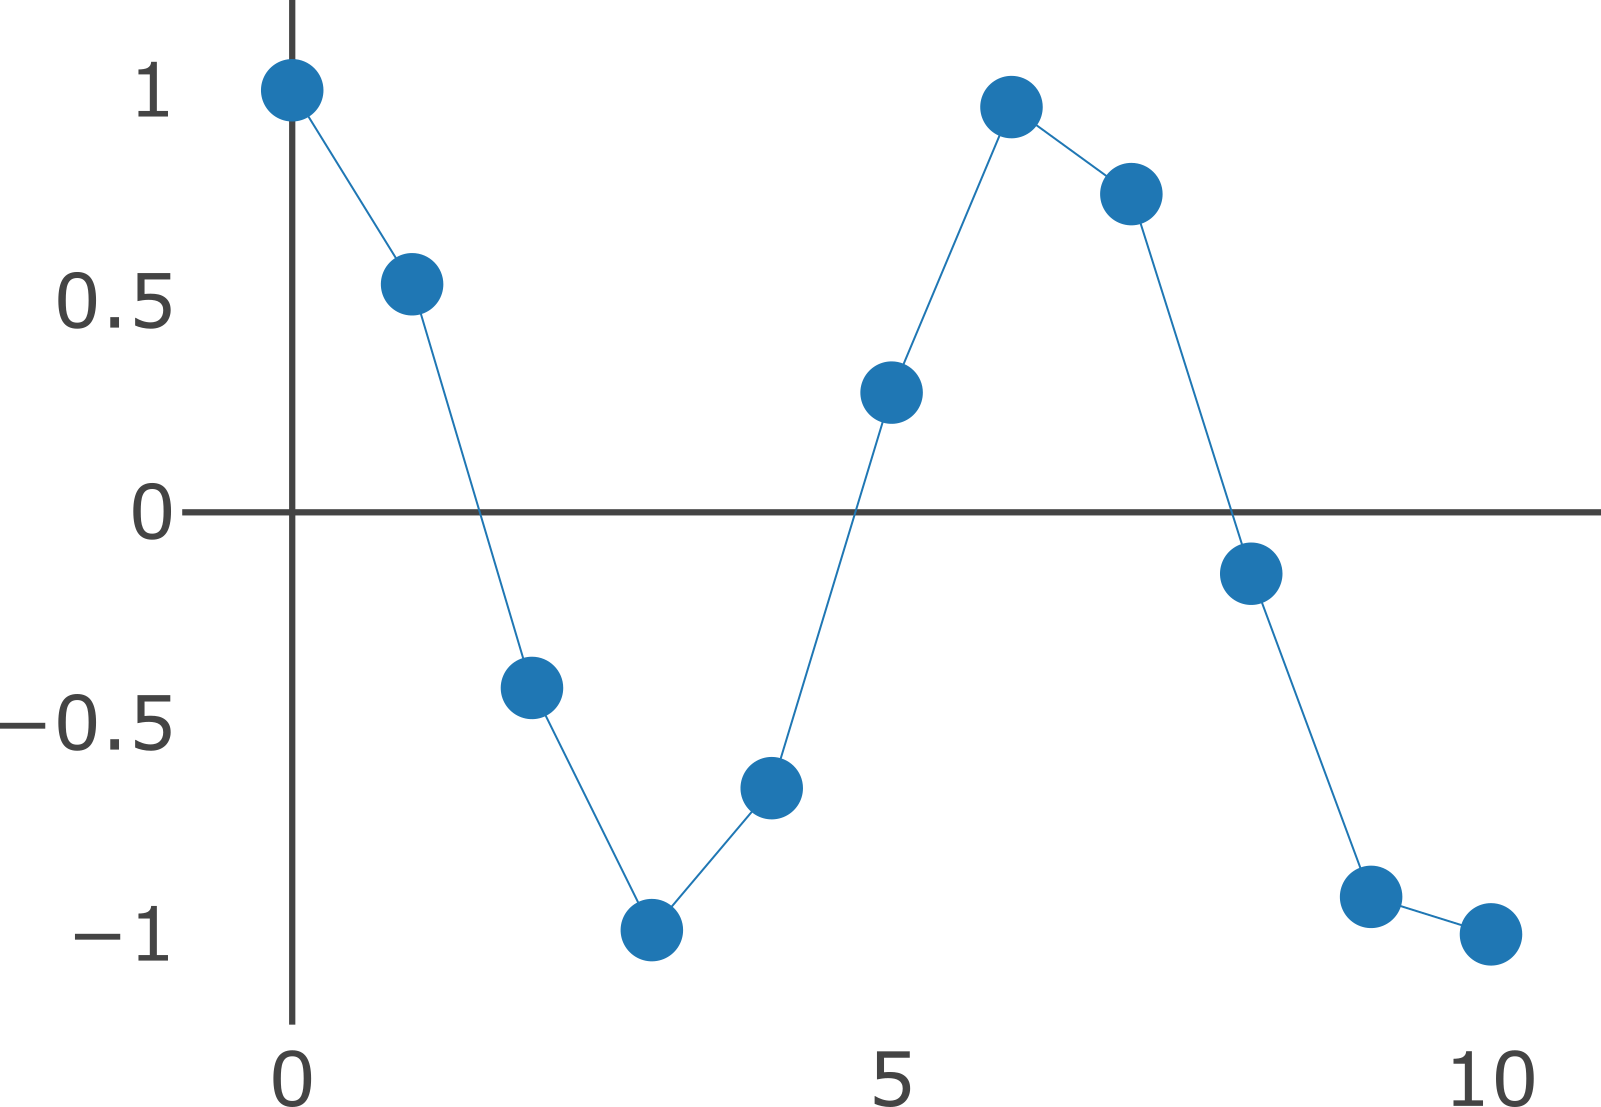
\includegraphics[width=.4\linewidth]{images/derivada} \hfill
  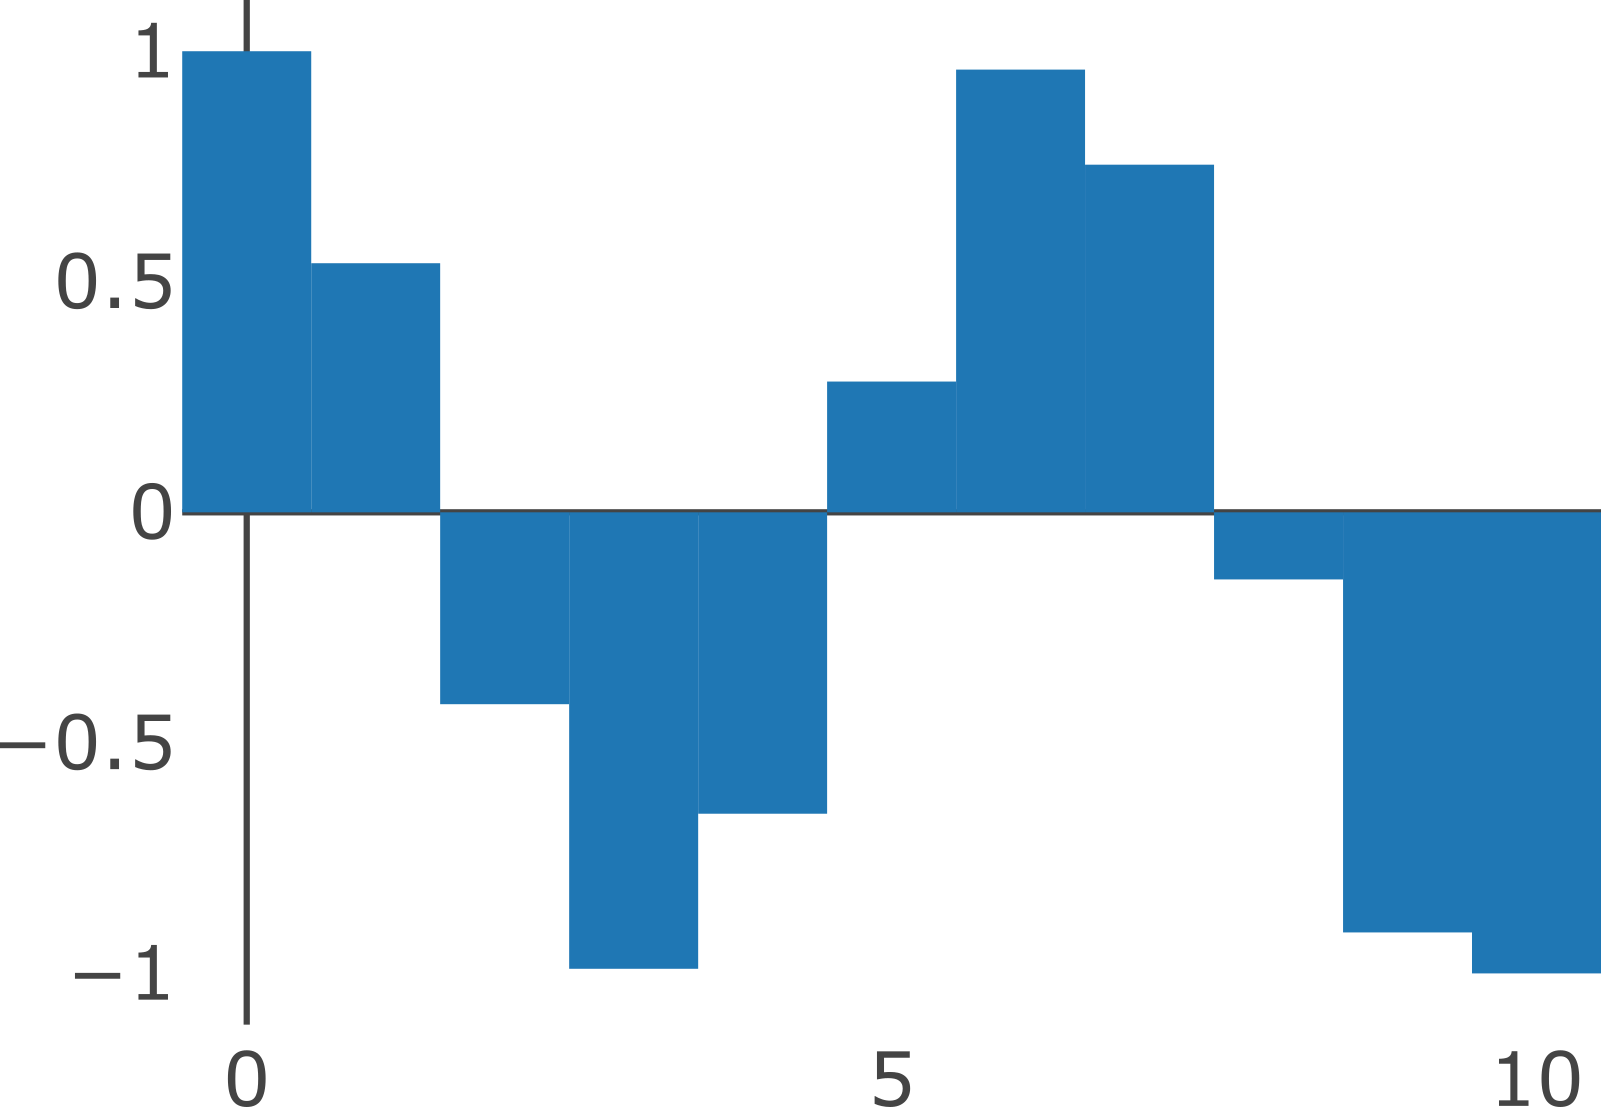
\includegraphics[width=.4\linewidth]{images/integral}
\caption{Interpretación de la derivada e integral.}
\label{fig:der_int}
\end{figure}


\subsection{Operador derivada}

\subsection{Integración con ParetoLib}
ParetoLib \cite{FORMATS_19, ParetoLib} es una librería de minería que recibe una especificación paramétrica o plantilla en STL y devuelve el rango de valores de las variables para las que la propiedad se satisface o invalida. 

Internamente, ParetoLib implementa un algoritmo de búsqueda que guía el aprendizaje y evalúa instancias concretas de la fórmula temporal a través de la herramienta STLEval.

% Contribuciones
En este proyecto, hemos actualizado los binarios y librerías dinámicas de STLEval que incorpora ParetoLib para dar soporte a las nuevas operaciones de derivación e integración. 
%TODO
%Referenciar a la rama de ParetoLib/GUI donde se engloban los cambios de la GUI + los nuevos binarios de STLEval

% Describir un ejemplo de STL con parametros sobre un operador derivada/integral?